\section{Splinter Design}
\label{sec:design}

Each Splinter server works as an in-memory key-value store
  (Figure~\ref{fig:arch}).
Like most key-value stores, tenants can directly \texttt{get} and \texttt{put} values, but they can also customize the
  store at runtime by installing safe Rust-based extensions (shared libraries mapped into the store's address space) (Figure~\ref{fig:arch} \textcircled{\footnotesize{1}}).
These extensions can define new operations on the tenant's data, including
  extensions that stitch together new data models in terms of the store's
  low-level get/put interface.
Each tenant-provided extension is exported over the network, so
  a tenant can remotely invoke the procedures it has installed into the store.

\begin{figure}[t]
  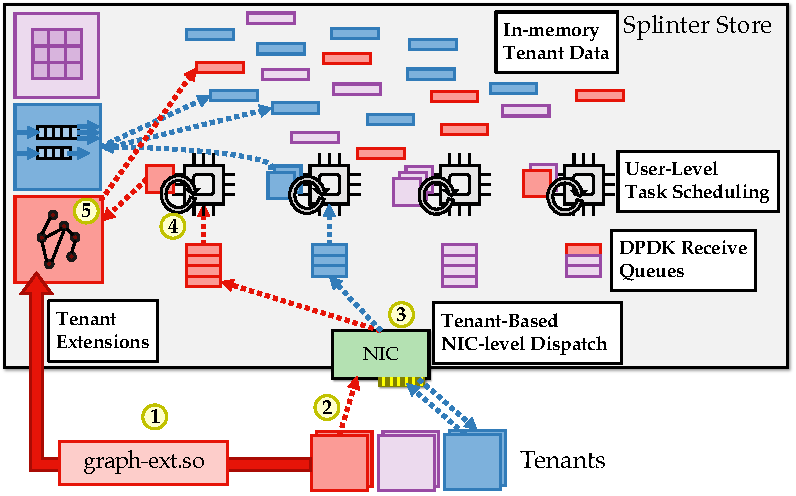
\includegraphics[width=1.0\columnwidth]{figures/splinter-arch.pdf}
  \caption{Overview of Splinter. Tenant data is stored in
  memory, and tenants can invoke extensions they have installed in the store (\textcircled{\footnotesize{1}}).
  Extensions are type safe, but compile to native code. The NIC uses
  kernel bypass for low latency (\textcircled{\footnotesize{2}}) and assists in dispatch by routing tenant
  requests to cores (\textcircled{\footnotesize{3}}). Each core runs
  a single {\sl worker} kernel thread that uses a user-level task scheduler to interleave
  the execution of tenant requests (\textcircled{\footnotesize{4}}).}
  \label{fig:arch}
\end{figure}


Tenants send requests to a Splinter store over the
  network using kernel bypass (\textcircled{\footnotesize{2}}).
Splinter currently only supports a simple, custom UDP-based RPC
  protocol, though other optimized transports may provide similar performance~\cite{erpc-arxiv}.
Each tenant's requests are steered to a specific receive queue by the
network
  card, improving locality (\textcircled{\footnotesize{3}}).
Each receive queue is paired with a single kernel thread (or {\sl worker}) that is pinned to a specific core.
Each worker pulls requests from its receive queue and creates a
user-level task for the requested operation.
Tasks provide an accounting
context for resources consumed while executing the
  operation, the storage needed to suspend/resume the
  operation, and a unit of scheduling.
Each worker has a task queue of new and suspended tasks, and it
  schedules across them to make progress in processing the operations
  (\textcircled{\footnotesize{4}}).
Scheduling is cooperative; as tasks yield and are resumed, they
store/restore their state, so when a worker
  schedules a task no stack switch is performed.
As tasks execute user-provided logic, they interact with the store through
  a \texttt{get}/\texttt{put} interface similar to the one exposed
  remotely (\textcircled{\footnotesize{5}});
the key difference is that the functions exposed to extensions
  take and return references rather than forcing copies (Table~\ref{table:db_interface}).

Beyond fast kernel-bypass network request processing, Splinter's speed depends on exploiting
  the Rust compiler in two key ways: first, to enable low-cost
  isolation and, second, to enable low-cost task switching.
The two are intertwined.
Splinter uses stackless generators to suspend and resume running
  extensions, which require compiler support.
That is, the Rust compiler analyzes extension code, determines the state that
  needs to be held across extension cooperative-yield/resume boundaries, and generates the
  code to suspend and resume extension operations.
No separate stack is needed, and the code needed to yield/resume is transparent
  to the extension.

These lightweight tasks are key, but Splinter's careful attention to object lifetimes, ownership, and memory safety
  make them effective, since otherwise full context switch would be needed between
  tasks for isolation.
A key challenge in Splinter is ensuring its fine-grained tasks from different
  trust domains---compiled to native code, and mapped directly into
  the store's memory---remain low-overhead while still operating within Rust's static
  safety checks.
Low-overhead trust boundary crossings are essential to Splinter's
  design;
they enable easy and inexpensive task switching, dispatch
(\S\ref{sec:coop}), and work stealing (\S\ref{sec:work-stealing}),
  which keep response latency low and CPU utilization high across all the cores
  of the store.

%Tenants' data and extensions must be isolated from one another, but using
%  hardware page tables and strong, physical separation of data is costly.
%Splinter avoids these costs by requiring extensions to be written in safe Rust.
%Splinter significantly lowers the cost of isolating extensions by requiring them to
%    be written in safe Rust.

Another key challenge is that extension invocations introduce more irregularity into request processing
  than a simple get/put interface.
%Some extensions operations may access many records or perform expensive
%  computation; others may only access a few records or probe an index.
By avoiding hardware context switches, Splinter keeps task switch costs down
    to about 11~nanoseconds, but the difficult tradeoff is that this forces
    it to handle these variable workloads without traditional
    preemptive scheduling.
At the same time, it cannot use fully cooperative scheduling, since the store
    does not trust tenants to supply well-behaved extensions.
Splinter's per-worker task scheduler resolves this tension by multiplexing
    long-running and short-running tasks to
    build mostly-cooperative scheduling.
This is backed up by having an extra thread that acts as a watchdog for the others to support
    preemption when needed.
%Splinter's reliance on Rust's type safety make this approach practical for
%  low-latency storage.
% 4.5 million invokes a second, 20% overhead ((1/4.5e6) * 0.2) * 1e9 -> 44 ns or so -> 44 ns @ 2.4 GHz -> 106 cycles.

\subsection{Compiling and Restricting Extensions}
\label{sec:compile}

The Splinter store cannot directly load native code provided by tenants.
Code must be compiled and type checked to ensure its safety before it can be
  loaded into a store, and extensions face some extra restrictions that must be
  enforced at compile time.
The compiler is trusted and must be run by the storage provider.
Tenants must not be able to tamper with the emitted extension, so it must be
  loaded directly into the store by the provider or the provider must
  ensure its integrity in transit between the trusted compiler and the store.
Aside from Rust's standard type and lifetime checks (\S\ref{sec:safety}),
  Splinter extensions have the following static restrictions:
  \begin{description}
    \item[No Unsafe Code.]
      Unsafe code could skip compiler checks resulting in memory unsafety.
      So, our wrapper over \texttt{rustc} disallows unsafe code in extensions
      (\S\ref{sec:unsafe}).
    \item[Module Whitelist.]
      Code from external dependencies could include unsafe code, and that
        unsafe code shouldn't be incorporated into untrusted extensions unless it
        is trusted.
      Even beyond memory safety, such unsafe blocks could, for example, make
        syscalls.
      So, our wrapper restricts external dependencies to modules that are
        re-exported by a Splinter library that includes many standard functions
        and types.
      This restriction applies to the standard library (\texttt{std}) as well: the
        wrapper only exposes whitelisted \texttt{std} functionality to extensions.
  \end{description}
These checks combine with three other runtime guarantees to
  ensure isolation:
the store only accepts or provides references to insert/fetch a value under a key
  if the same tenant owns both the extension and the key (\S\ref{sec:db-iface});
it prevents uncooperative extensions from dominating CPU time and stack, heap, or record memory (\S\ref{sec:coop}); and
it catches panics (runtime exceptions) and stack overflows that occur while executing an
  extension operation (\S\ref{sec:coop}).
Next, we describe what guarantees this gives the storage provider and its tenants;
  the runtime checks are described later along with details about the execution model.

\subsubsection{Trust Model}
\label{sec:trust}

There are two stakeholders for a Splinter store: the storage
provider and storage tenants. Splinter should protect tenants from each other
and the provider from the tenants. Tenant
misbehavior could be unintentional, in the form of bugs or unexpectedly high
application load, or it could be malicious, in the form of tenants attempting
to read others' data, deny service, or use an unfair fraction of resources.
We consider threats from ``within'' the store; threats from ``without'' such
as an attacker gaining root access to the machine by exploiting other services
running on it should be dealt with using standard security best practices.

%A store hosting Splinter extensions needs to protect the store itself from
%tenant-provided extensions and it needs to protect extensions from one another.
%Splinter is designed for two main use cases: one where the store and its
%extensions come from a single organization, and a pure multi-tenant environment
%where extensions are untrusted by the store, mutually distrusting, and
%potentially adversarial. In both cases, there are two key types of
%stakeholders: storage providers and storage tenants.

Aside from providing good quality of service to tenants, service providers
  have one key concern: protecting the secrecy and integrity of tenants' data.
Extensions don't share state with one another, and Splinter provides no means for
inter-extension communication. So, no complex sharing policies are needed;
Splinter's only goal is extension isolation.
Rust references act as capabilities; they ensure that extensions cannot
fabricate arbitrary references
to storage state or to other tenants' state~(\S\ref{sec:safety}).

Like any database, Splinter's Trusted Computing Base (TCB) includes the
    libraries, compilers, hardware, etc.\ on which it is built; while
    this code is not directly exposed to tenants, vulnerabilities in it can
    still lead to exploits.
Dependencies include LLVM~\cite{llvm}, the CPU, the 
    network card (NIC) and its kernel-bypass libraries (DPDK~\cite{dpdk}).

Splinter's design provides a larger attack surface relative to other
    databases in some ways, but decreases the attack surface in others.
Because it allows execution of tenant code, Splinter's safety depends on the
    soundness of Rust's type system, which is not proven.
While some soundness issues in the compiler have been
    found~\cite{rustc-unsound}, progress is being made in proof
    efforts~\cite{rustbelt-2018}, and Splinter automatically benefits from
    such progress.
If extensions cannot violate Rust's safe types, the remaining avenue for
    attack is unsafe code in the system; extensions cannot supply unsafe
    code, but they can indirectly call it in the 
    interfaces and libraries that Splinter explicitly exposes to extensions.
On the plus side, extensions \emph{must} break one of these layers of
    protection before they can attack other code: they do not have
    direct access to system libraries, system calls, etc.\ and can only gain it
    by breaking out of Rust's safe environment.

Splinter decreases the attack surface with respect to the virtual memory system --
    both hardware and kernel components.
Because it doesn't rely on virtual address translation for
    isolation,
    recent Meltdown speculation attacks don't affect its design~\cite{meltdown-2018}%
%\old{; however, it must use compiler mitigation against recent attacks on speculatively
    %executed indirect branches~\cite{spectre-2018,llvm-spectre}.}%
; however, Spectre-based speculation attacks do affect Splinter~\cite{sbo,spectre-2018}.
Like any system that runs untrusted code or operates on untrusted
  inputs, Splinter would require special steps to mitigate these side channels.
It already limits them in part because it doesn't provide explicit
  timing functions to extensions.
Full protection will require compiler support~\cite{llvm-spectre},
hardened storage interfaces (like
  the Linux kernel~\cite{linux-spectre}), and hardened libraries for
  extensions.
The measurements in this paper do not include these mitigations.

\subsubsection{Memory Safety}
\label{sec:safety}

Rust's memory safety (and data race freedom) is guaranteed through a strong notion
  of \textsl{ownership} that lets the \texttt{rustc} compiler reason statically
  about the lifetime of each object and any references to it.
The compiler's \textsl{borrow checker} statically tracks where objects and
  references are created and destroyed.
It ensures that the lifetime of a reference (initially determined by its binding's scope)
  is subsumed by the lifetime of its referent.
Rust separates immutable and mutable references; an immutable reference is a
  reference that when held restricts access to the underlying object to be read-only.
The compiler disallows multiple references (of either type) to
  an object while a mutable reference exists, which prevents data races.

Often, the lifetime of an object cannot be restricted to a single, static scope.
This is especially true in a server that processes requests across threads,
  where the lifetime of many objects (RPC buffers, extension runtime
  state) is defined by request/response.
Rust provides various accommodations for this, such as moving ownership between
  bindings and runtime reference counting that is safe but implemented in unsafe Rust.
Splinter efficiently handles these issues while working within
\texttt{rustc}'s static safety checks (\S\ref{sec:access}).
Unlike C/C++ pointers, Rust references cannot be fabricated or manipulated with
  arithmetic; they always refer to a valid, live object.
Rust supports pointers but their use is restricted for safety.

\subsubsection{Restricting Unsafe Rust}
\label{sec:unsafe}

An important extra restriction that Splinter imposes beyond Rust is that
  extension code must be free from \emph{unsafe} Rust, a superset of the
  language that allows
  operations that could violate its safety properties.
For example, unsafe code can dereference pointers, perform unsafe casts, omit
  bounds checks, and implement low-level synchronization primitives.
All unsafe code in Rust requires an \texttt{unsafe} block, which
Splinter disallows in extension code.

Extensions cannot implement unsafe code, but they can invoke it indirectly.
This is often desired.
For example, extensions execute some unsafe code when they ask the store to
  populate a response packet buffer.
In some cases it is not desired.
For example, file I/O can be induced through the Rust standard
  library.
To prevent this, Splinter restricts extensions to use a subset of the standard
  library that doesn't include I/O or OS functionality.

Our experience has been that safe Rust combined with basic data structures from
  its standard library are sufficient to write even complex imperative extensions
  like Facebook's TAO~\cite{tao-2013}.
In cases where unsafe code could provide a performance benefit, the store can
  provide that functionality if it is deemed safe to do so, since it is trusted
  and can include \texttt{unsafe} code (\S\ref{sec:ser-des}).

\subsection{Store Extension Interface}
\label{sec:db-iface}

\begin{table}[t]
\caption{Extensions interact with the store locally through an interface designed to
  avoid data copying.}
\centering
\begin{tabular}[]{l c c}
\toprule
\textbf{Store Operations for Extensions} \\
\midrule
\textbf{get}(table: u64, key: \&[u8]) $\rightarrow$ Option$\langle$ReadBuf$\rangle$ \\
  \hspace{1em} Return view of current value stored under $\langle$\texttt{table}, \texttt{key}$\rangle$. \\
  \\
\textbf{alloc}(table: u64, key: \&[u8], len: u64) $\rightarrow$ Option$\langle$WriteBuf$\rangle$ \\
  \hspace{1em} Get buffer to be filled and then \texttt{put} under $\langle$\texttt{table}, \texttt{key}$\rangle$. \\
  \\
\textbf{put}(buf: WriteBuf) $\rightarrow$ bool \\
  \hspace{1em} Insert filled buffer allocated with \texttt{alloc}. \\
  \\
\textbf{args}() $\rightarrow$ \&[u8] \\
  \hspace{1em} Return a slice to procedure args in request receive buffer. \\
  \\
\textbf{resp}(data: \&[u8]) \\
  \hspace{1em} Append data to response packet buffer. \\
\bottomrule
\end{tabular}
\label{table:db_interface}
\end{table}

The interface that extensions use on the server to interact with stored records is similar to
  the external, remote interface that clients use in any conventional key-value
  store (Table~\ref{table:db_interface}).
The main differences are in careful organization to eliminate the need to copy
  data between buffers.

All persisted records are stored in a \emph{table heap}.
Keeping records in a identifiable region will be essential to support
  replication, recovery, and garbage collection as Splinter's implementation
  evolves.

\subsubsection{Storing Values}

Extensions can \texttt{put()} data they receive over the network
  or new values that they produce into the store.
%Both are handled in the same way. 
When an extension invocation request is received from a tenant, the store invokes the indicated operation.
Incoming data is in a packet buffer that is registered with the NIC.
Those buffers cannot be used for long-term storage
  because the NIC must use them to receive new requests;
data that must be preserved needs to be copied into the store.

Splinter tries to ensure that data can be moved from NIC buffers into the
    store with a single copy.
This requires \texttt{put()} to be split into two steps.
First, an extension calls \texttt{alloc(table, key, length)} to allocate a region in
  the table heap for a record.
The extension receives a bounded slice (a view) to the underlying allocated
  memory.
Then, it copies data from the request's receive buffer, unmarshalling
    as it does so, if needed.
Extensions use \texttt{args()} to directly access data (by
  reference) in the receive buffer to perform this copy.
An extension may produce its own data values as part of this process
    either from input arguments or together with values read from the store.
Once the allocated region is properly populated, it is inserted into the
  table with \texttt{put()},
which takes ownership of the buffer and inserts it into a hash table.

Problems like use-after-free are prevented by Rust's borrow checker;
extensions cannot hold references to a buffer once ownership is
  transferred to the store, eliminating the need for copying data into the
  store for safety.
The receive packet buffer has the same guarantee.
Rust's borrow checker ensures references to it cannot outlast
  the life of the RPC, eliminating the need to copy
  received arguments or data into the extension for safety.

Values stored by \texttt{put()} must be allocated from the table heap;
  extensions should not be able to pass arbitrary (heap or stack allocated)
  memory to \texttt{put()}.
Splinter enforces this so that it can optimize record layout;
keys and values can be forced into a single table heap allocation, which
  eases heap management and eliminates cache misses for hash table lookups.
As a result, Splinter wraps allocations
  with a type (\texttt{WriteBuf}) that extensions cannot construct,
  ensuring they can
  only pass buffers acquired from \texttt{alloc()}.
\texttt{WriteBuf} has a method to get a reference to the
  underlying buffer, so extensions can fill it.

\subsubsection{Accessing Values}
\label{sec:access}

Extensions can interact with stored data in a similar way, requiring only one
  copy into a response buffer to return values from the store.
When an extension procedure is invoked, it is also provided with a response
  buffer that can be incrementally filled via \texttt{resp()}.
On each extension procedure invocation, the store pre-populates the response
  buffer's packet headers; extensions can only append their data after these
  headers.
All response buffers are pre-registered with the NIC for transmission.

\begin{figure}[t]
\centering
\begin{lstlisting}[language=C++]
fn aggregate(db: Rc<DB>) {
  let mut sum = 0u64;
  let mut status = SUCCESS;
  let key = &db.args()[..size_of::<u64>()];

  if let Some(key_lst) = db.get(TBL, key) {
    // Iterate KLEN sub-slices from key_lst
    for k in key_lst.read().chunks(KLEN) {
      if let Some(v) = db.get(TBL, k) {
        sum += v.read()[0] as u64;
      } else {
        status = INVALIDKEY;
        break;
      }
    }
  } else {
    status = INVALIDARG;
  }
  db.resp(pack(&status));
  db.resp(pack(&sum));
}
\end{lstlisting}
\caption{Example aggregate extension code. The extension takes a key as
input (directly from a request receive buffer), looks it up in the
store, and gets a reference to a value that contains a list of keys. It
looks up each of those keys, it sums their values, and directly appends
the result to a response buffer.}
\label{lst:aggregate}
\end{figure}

Extensions call \texttt{get(table, key)}, and they receive back a reference to
  the underlying portion of the table heap that contains the value associated
  with \texttt{key}.
No copying is needed at this step; the store tracks this reference and prevents the table
  heap garbage collector from freeing the buffer while an extension has a live
  reference to the data.
Since values are never updated in place, extensions see stable views of values.
Extensions can compute over the value or many values concurrently (by calling \texttt{get()} multiple times), and they can
  copy portions of the data they observe or any results they compute directly into
  the response buffer.
Once the extension procedure has populated the response buffer, Intel's
  DDIO~\cite{ddio} transmits the data directly from the L1 cache, which avoids
  the cost of memory access for DMA of stored data.

\begin{figure}[t]
  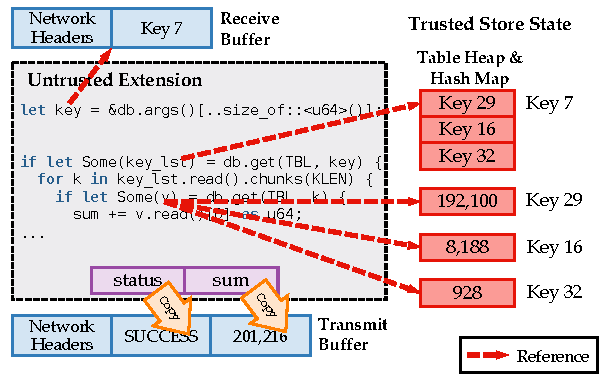
\includegraphics[width=1.0\columnwidth]{figures/tao-extension.pdf}
  \vspace{2pt}
  \caption{References during aggregation. All data accessed by the extension in
  Listing~\ref{lst:aggregate} is by reference whether that data is part of the
  arguments in the receive buffer or part of a record in the store. References
  work in reverse for the response; the extension passes references to data to
  the store, and the store copies that data into the response buffer.}
  \label{fig:tao}
\end{figure}


Listing~\ref{lst:aggregate} and Figure~\ref{fig:tao} show an example of how
  this works for a simple extension that sums up a set of values stored under
  keys that are listed as part of another stored value without any extra data copying.
In Line~4, the extension obtains a reference to its transmit buffer to find
  which key it should look up in order to find a list of keys that will be aggregated over.
Line~6 passes a reference to that same location to the store in order to
  obtain a reference to the value that contains the key list.
In Line~8, still without copying, the extension iterates over that value in
  chunks equal to the length of the keys stored in the value.
Each step of the iteration produces a reference that the extension uses
to \texttt{get()}
  references to values for each of the stored keys, one at a time (Line~9).
Using each of those references, it extracts a field that it adds to
  \texttt{sum}, a local variable.
Finally, the extension passes references to \texttt{status} and \texttt{sum} to append
  them to the response buffer.
In all, data copying is only forced where it is needed, so the compiler has
  flexibility in optimizing extension code.

The store's \texttt{get()} call returns a \texttt{ReadBuf} rather than a plain
  slice (\texttt{\&[u8]}) in order to satisfy Rust's borrow checker.
Calling \texttt{get()} cannot return an immutable reference or slice to a stored
  value, because the borrow checker wouldn't be able to statically verify that the
  reference would always refer to a valid location.
For example, the compiler couldn't be sure that the store wouldn't garbage
  collect the value while the reference still exists.
Furthermore, extension invocations are generators, and they must
  yield regularly (\S\ref{sec:coop}).
Yielding marks the end and start of a new static scope, so
  each time the generator is resumed, the calling scope could vary.
Any obtained references to a stored value couldn't be held across yields,
  because the borrow checker wouldn't be able to verify that those
  references would still be valid on reentry.
%In the end, this would complicate extension code and would force extensions make
  %additional \texttt{get()}s to ensure Rust could verify memory
  %safety.}

The \texttt{ReadBuf} returned by \texttt{get()} solves this.
It is a smart pointer that maintains a reference count to ensure
  the underlying stored object isn't disposed, and it allows the extension code
  to (re-)obtain a reference to the underlying object data.
Once a \texttt{ReadBuf} is returned to a generator, it is stored within the
  generator's local state, so the generator owns this \texttt{ReadBuf}.
Extensions cannot hold references between yields,
  but by working with the \texttt{ReadBuf} it can (transparently) re-obtain a
  reference to the data without performing another \texttt{get()}.
Rust's \texttt{Arc} smart pointer does the same;
  \texttt{ReadBuf} hides its constructor from extensions and disallows duplication.
This prevents extension code from creating \texttt{ReadBuf}s that persist
  beyond the life of a single request/response, which could otherwise hold back
  table heap garbage collection.

\subsubsection{Avoiding Serialization and De-serialization}
\label{sec:ser-des}

Allowing extensions to interact directly with receive buffers, transmit buffers,
  and table heap buffers eliminates copying for opaque data, but Rust's safety
  makes avoiding some copies harder.
Extensions cannot perform unsafe operations, otherwise they could thwart Rust's
  memory safety guarantees.
Unfortunately, this means safe Rust code cannot cast an opaque byte array to/from
  different types to avoid the need to serialize/de-serialize data.
For example, if \texttt{args()} returned an 8-byte slice an extension may desire
  to treat that slice data as a 64-bit unsigned value.
Safe Rust disallows this.

For small arguments, extensions can convert between
  formats with arithmetic, but for richer data models, arguments, stored values, and responses will
  have more complex, structured formats.
To accommodate this, Splinter's interface provides a mechanism for extension
  code to convert between byte slices and references to a small set of types.
If a slice (\texttt{\&[u8]}) is naturally aligned to the desired
  type, Splinter allows conversion to a reference of that type
  (\texttt{\&T}), where \texttt{T} is limited to signed/unsigned
  integers and compound types built from them.

These casts are safe, but they are meaningless across architectures. As a
  result, they can only be used between a client and the store when they have
  the same underlying platform (e.g.\ x86-64).
Similarly, they can only be used with extensions'
  \texttt{get}/\texttt{alloc}/\texttt{put} interface if all stores in
  the system (e.g.\  before/after recovery, source/destination for migration) have matching hardware
  platforms.

\subsection{Cooperatively Scheduled Extensions}
\label{sec:coop}

Splinter is designed to work well regardless of whether tenant-provided
  extensions are short and latency-sensitive or long-running and compute- or
  data-intensive.
In fact, the best mix of tenants will mix these operations, keeping CPU,
  network, and in-memory storage better utilized than would be possible with a
  single, homogeneous workload.
Even so, latency-sensitive operations can easily suffer under interference from
  heavier operations.

This means Splinter must multiplex execution of tenant extension invocations
  not only across cores but also within a core.
Long-running procedures cannot be allowed to dominate CPUs, but
  preemptive multitasking is too costly even when page table switching can
  be avoided.

Rust's lightweight isolation is part of the solution, since calls across
  trust domains have little overhead.
Splinter already relies on \texttt{rustc} for safety, but it can also rely on
  it to help minimize task switching costs.
When a new request comes into the store, Splinter calls into the responsible extension
  to allocate a stackless coroutine (a generator) that closes
  over the state needed to process the request.
Generators support a
  \texttt{yield} statement that suspends execution and enables
  cooperative scheduling;
  extension code is expected to periodically call \texttt{yield} to
  allow other tasks to run.
\texttt{rustc} produces generators specific to the extension, so the
  cost to create them and switch between them is low.
Splinter invokes the created generator.
Whenever it yields,
  Splinter's per-core task scheduler runs another generator task.
Since yielding requires no costly hardware boundary crossing and no stack
  switch, it is fast and inexpensive to yield frequently.

%Splinter use stride scheduling~\cite{stride,bvt} on virtual time and a priority
%  queue to schedule tasks.
%Short-running tasks complete quickly, and longer-running tasks lose priority to
%  fresh, incoming tasks but naturally avoid starvation as they age.
%Yield is inexpensive, so tasks that yield frequently aren't punished and
%  maintain high priority.

Like other similar systems, to avoid jitter due to kernel thread context
    switches and migrations, Splinter runs
    the same number of
  worker threads as cores in the system (Figure~\ref{fig:arch}), and each is
  pinned to a specific core.
Generators are invoked on the worker's stack, avoiding a stack switch.
Note that the compiler generates the structure to hold a suspended
  task's state across yields.
Consequently, a worker's stack never concurrently contains state for
  different tenants (or even tasks); furthermore, whenever a task
  yields or completes, the worker's stack contains no extension state.
This makes it easier to handle uncooperative extensions (\S\ref{sec:uncoop})
  and load imbalance (\S\ref{sec:work-stealing}).

\subsubsection{Uncooperative and Misbehaving Extensions}
\label{sec:uncoop}

All calls through the store interface include an implicit yield, so extensions
  can only dominate CPU time with infinite or compute-intensive loops.
Nonetheless, such behavior can disrupt latency-sensitive tasks and constitute a
  denial-of-service attack in the limit.

To solve this, Splinter uses ideas from user-level threading for
  latency-sensitive services~\cite{arachne-2018} and adapts them for
  untrusted code.
An extra (mostly idle) thread acts as a watchdog.
If a task on a core fails to yield for a few milliseconds, the watchdog
  remedies the situation.
First, the worker thread on the core with the uncooperative task is
  re-pinned to a specific core that is shared among all misbehaving threads
  and low-priority background work that the store performs.
Second, a new worker kernel thread is started and pinned to the idle core left behind
  after the misbehaving thread was re-pinned.
Finally, the new worker steals the tasks remaining in the scheduler queue for
  the re-pinned worker and resumes execution for these tasks.
Note, this is safe in part because all of the state of a suspended task is
  encapsulated.
Tasks only have state on a worker's stack if they are running, so
  the misbehaving task is the only one the new worker cannot steal.
Whenever a misbehaving task finally yields, the scheduler on that worker realizes
  that it has been displaced, and the worker thread terminates along with the task.

Hence, misbehaving tasks don't block other requests, but they can still cause
  disruption.
Creating and migrating kernel threads is expensive,
  so there must be a disincentive against forcing watchdog action.
Tenants that run uncooperative tasks will experience poor quality of
  service, since they must share a core with other disruptive
  work.
Furthermore, when a worker is re-pinned the watchdog also takes away access to its
  receive and transmit queues, so tenants cannot get responses from bad
  requests and, thus, benefit from their misbehavior.
% \textbf{Can you take away their ability to \texttt{put()} too?} % We can do this, but we don't yet -- we should put this is shortly after deadline.
Even so, billing policies should ensure such behavior is unprofitable.

Aside from infinite loops, the store must also
  protect against other things that cannot be prevented with compile-time checks.
For example, Rust doesn't have general exceptions, but
  extensions can raise exceptions with operations like division by
  zero that raise a \texttt{panic}.
Splinter must ``catch'' these panics or they would terminate the worker,
  since panics unwind the call stack and worker threads call
  extension code on their own stack.
Fortunately, Rust provides a mechanism to do this, and Splinter catches
    panics and converts them to an error response to the appropriate client.
Stack overflows and violation of heap quotas are handled similarly.

\subsection{Tenant Locality and Work Stealing}
\label{sec:work-stealing}

The Splinter store avoids any kind of centralized dispatch core to route
  requests to cores, since this can easily become a bottleneck~\cite{ramcloud}.
At the same time, it needs to balance requests across cores, while still trying
  to exploit locality to avoid cross-core coordination overheads.
To do this, clients route each tenant's requests to a particular core.
This provides cache locality, it reduces contention, and it improves performance
  isolation.
Splinter configures Flow Director~\cite{flow-director} so that
  the NIC directly stores packets with a specific destination port
  number in a specific
  receive queue.
Each receive queue is paired to a single task dispatcher owned by a
worker thread (pinned to a core).
As a result, tenants can steer requests to specific cores by placing their
  tenant id in the UDP destination port field.

\begin{figure}[t]
  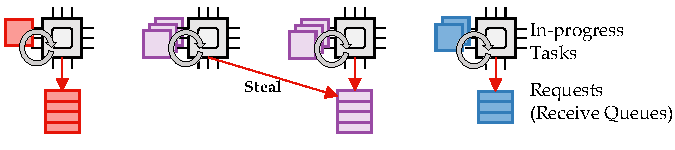
\includegraphics[width=1.0\columnwidth]{figures/work-stealing.pdf}
  \caption{Dispatch tasks on each core steal requests from the receive queue of
  the core to their right whenever they have no requests in their own
  receive queue. As a result, work from
  overloaded cores get redistributed without generating high contention. Here,
  core 1's in-progress tasks were induced by requests stolen from
  core 2's queue.}
  \label{fig:work-stealing}
\end{figure}


However, this approach alone can leave cores idle under imbalance, and, as a multi-tenant
  store, it is important for the system to deliver good resource utilization.
Whenever the scheduler on a core has no
  incoming requests in its local receive queue, it attempts to steal requests
  from a neighbor's receive queue (Figure~\ref{fig:work-stealing}).
Transmit queues aren't bound to specific (server-side) source ports, so the
  response can be sent directly from the core that stole the request.
This simple form of soft affinity works well, and, since tasks are lightweight,
  it is also relatively easy for Splinter to take advantage of idle compute
  in the system without costly thread migration.
